% Když budete cokoli psát: ukládejte starší verze vždy odděleně, abyste se 
% k nim mohli kdykoli vrátit. Kusy textu, které jste se rozhodli nepoužít, taky ukládejte do zvláštního souboru. Smazat se to dá vždycky, ale psát to znova je opruz. 

% A POŘÁD ZÁLOHUJTE. POŘÁD !!!

\usepackage{extsizes}
\documentclass[17pt]{extreport}
%\documentclass[12pt, a3paper, oneside]{article} 
% velikost písma, stránky, typ dokumentu -- detaily viz literatura

\usepackage{czech} % nastavení češtiny
%\usepackage[latin2]{inputenc}
%\usepackage[cp1250]{inputenc} % pro win1250
\usepackage[utf8]{inputenc}
\usepackage{wrapfig} % nastavení obtékání textu
\usepackage{graphicx,amsmath} % nastavení grafiky, matematiky
\usepackage{subfig} % více obrázků vedle sebe 
\usepackage{float}
\usepackage{amsmath}
\usepackage{fix-cm}
\usepackage{amssymb}
\usepackage{bbding}
\usepackage{enumitem}
\usepackage{multicol}
\usepackage{xfrac}
\usepackage[a3paper]{geometry}
\usepackage{tocloft} %přidá tečky do obsahu ke kapitolám /sekcím 
\usepackage{pdflscape}
\usepackage{wrapfig}
\renewcommand{\cftsecdotsep}{\cftdotsep}

\usepackage[bookmarksopen,colorlinks,plainpages=false,linkcolor=black,urlcolor=blue,citecolor=black,filecolor=black,menucolor=black,unicode=true]{hyperref}
%bookmarksopen -- open up bookmark tree 
%colorlinks -- zbarví odkazy (implicitně orámovaný nezbarvený text)
%urlcolor -- barva odkazů (implicitně magenta) 
%linkcolor=black -- barva odkazů v obsahu (implicitně red)


\usepackage{listings}
\usepackage{color}
\definecolor{lightgray}{rgb}{.9,.9,.9}
\definecolor{darkgray}{rgb}{.4,.4,.4}
\definecolor{purple}{rgb}{0.65, 0.12, 0.82}

%\usepackage{parskip} %-- zapne americké odstavce v celé práci

\setlength{\textwidth}{250mm}
\setlength{\hoffset}{-20mm}  % posun textu kvůli kroužkové vazbě  


\setlength{\intextsep}{5mm} % nastavení mezery okolo obrázků

% nastavení příkazu >\figcaption pro popis čehokoli, jako by to byly obrázky 
\makeatletter   
\newcommand\figcaption{\def\@captype{figure}\caption}
\makeatother

% přejmenuje anglický název Reference na české Literatura


%\makeindex % příprava pro výrobu indexu (jestli ho chcete)

%%    VLNKA <fileinput>  KkSsVvZzOoUuAaIi        
% Defaultni  koncovka pro <fileinput> je  ".tex"
%FIXME: haze error
%\cstieon % Vypne chovani vlnky jako tvrde mezery v matematickem rezimu

%%%%%%%%%%%%%%%%%%%%%%%%%%%%%%%%%%%%%%%%%%%%%%%%%%%%%%%%%%%%%%%
%V PROSTŘEDÍ ROVNIC SE NESMÍ VYSKYTOVAT PRÁZDNÝ ŘÁDEK
%
%PROGRAMY VLNKA A CSINDEX SE MUSÍ SPUSTIT SAMOSTATNĚ
%%%%%%%%%%%%%%%%%%%%%%%%%%%%%%%%%%%%%%%%%%%%%%%%%%%%%%%%%%%%%%%

% definice příkazů 
\newcommand{\D}{\medskip \noindent} % nový odstavec v "americkém" formátování 
\newcommand{\B}{\textbf} %tučné písmo
\newcommand{\A}{\mathbf} %tučné písmo v matematickém režimu
\newcommand{\TO}{\ensuremath{\boldsymbol\Omega}} % tučný znak velké omega -- pro ohmy
\newcommand{\I}{\index}  % vytváří položku indexu (asi nepoužijete)
\newcommand{\Deg}[1][]{\ensuremath{{#1}^\circ}} % vysází značku stupně Celsia
\newcommand{\Def}{\footnotesize Definice: \normalsize}
\newcommand{\Pos}{\footnotesize Experiment: \normalsize}
\newcommand{\Odv}{\footnotesize Odvození: \normalsize}
\newcommand{\Vym}{\footnotesize Vymezení pojmu: \normalsize}
\newcommand{\Ob}{}
\newcommand{\It}{\textit}  % kurzíva
\newcommand{\M}{\mathrm}   % v prostředí rovnic nastaví normální písmo (místo kurzívy ) 
\newcommand{\F}{\footnotesize} % zmenšená velikost písma
\newcommand{\N}{\normalsize} % normální velikost písma
%\newcommand{\U}{\underline}  % podtržené písmo
\newcommand{\e}{\ensuremath} 
\newcommand{\Has}{\textcolor{green}{\CheckmarkBold}}
\newcommand{\NoHas}{\textcolor{red}{\XSolidBrush}}
% další příkaz se aplikuje, pouze, když jste v matematickém režimu

%\hyphenation{Pusť-me pla-tí hod-no-ty do-sa-dí-me za-da-né dal-ším}
% dělení slov, kdyby implicitní nevyhovovalo

\linespread{1.0} 
% řádkování 1,5x  
% použijete podle situace  

\unitlength=1mm % nastavení volby jednotek 


% konec hlavičky
%%%%%%%%%%%%%%%%%%%%%%%%%%%%%%%%%%%%%%%%%%%%%%%%%%%%%%%%%%%%%%%%%%%
%%%%%%%%%%%%%%%%%%%%%%%%%%%%%%%%%%%%%%%%%%%%%%%%%%%%%%%%%%%%%%%%%%%

\begin{document} % začátek textové části 

% titulní strana
\pagestyle{empty} % vynechá číslování

\voffset = -20mm % posun začátku textu výš
\enlargethispage{100mm} % zvětší oblast tisku pro tuto stránku   

\begin{center}
    \Large \B{LORRIS TOOLBOX \\ Set of tools designed for developement\\and controling of robots}
\end{center}
\vspace{5mm}
\setlength{\footskip}{0pt}
\setlength{\textheight}{750pt}
Lorris Toolbox is a suit of multiple tools, which all share the same goal -- to help with developement, debugging and controling of not only robots, but also other electronic devices. \\ \\
{\large \B{ 1. Analyzer }}
\begin{figure}[ht]
    \begin{minipage}[t]{0.48\linewidth}
    \begin{itemize} 
        \item It's main purpose is to graphically display the data from robot.
        \item Analyzer uses widgets to display data -- small \uv{windows}, each showing certain part of data.
        \item Each widget has individual settings and the user can place them anywhere on the workspace.
        \item Using widgets, it is possible to assemble interface suitable for virtually any robot.
        
    \end{itemize}
    \end{minipage}
    \hfill
    \begin{minipage}[t]{0.50\linewidth}
    %\subfloat{
        \vspace{0pt}
        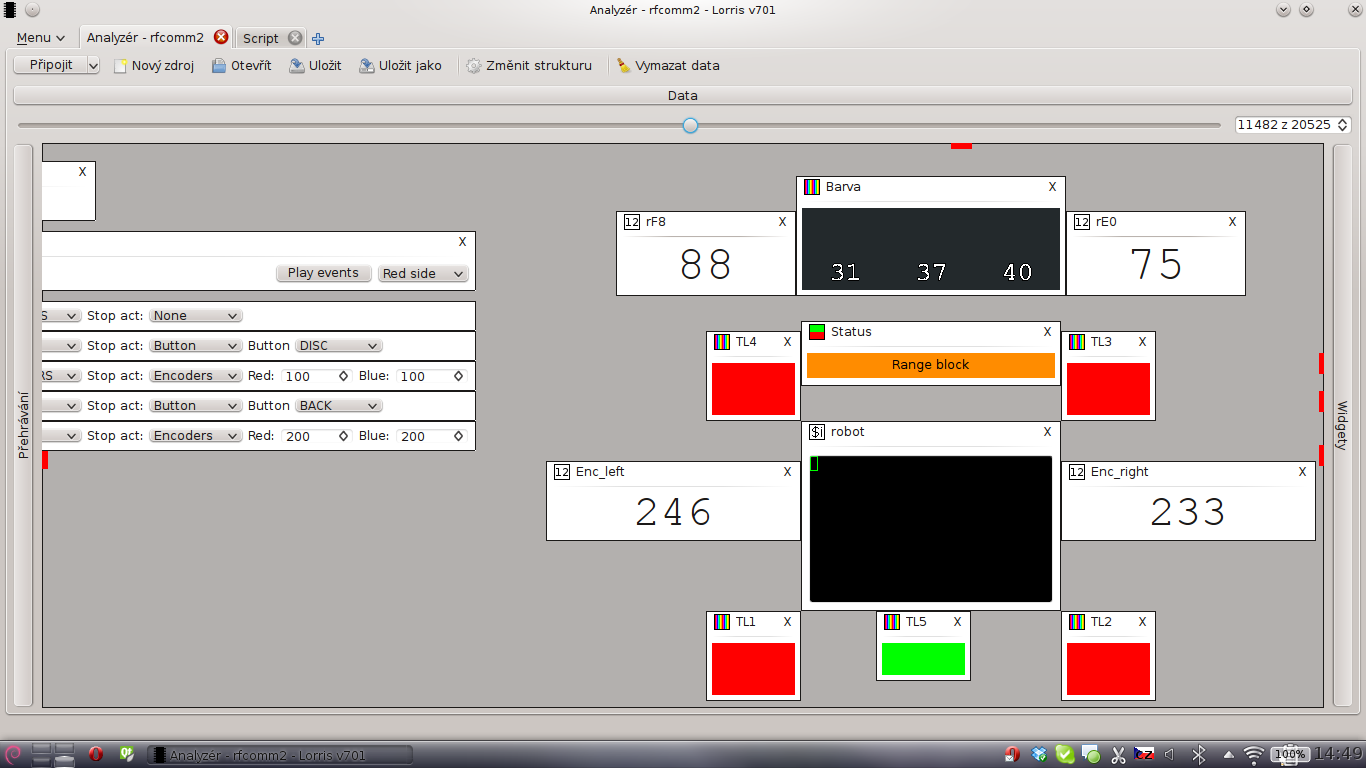
\includegraphics[width=\linewidth]{img/screen.png}
        \centering \It{Main application window}
    %}
    \end{minipage}
\end{figure}
\vspace{-7mm}
\begin{itemize} 
    \item Multiple types of widgets are available in Lorris, for example \It{Number, Color, Column bar, Circle} (displaying angle within circle) or \It{Graph}.
    \item Analyzer is also ideal for easy displaying of data from components for which using only numbers is not eligible, e.g. color sensor.
    \item Some widgets can also send data to the robot. This means that beside displaying data, widgets can also control the robot.
    \item Of all the widget types, \uv{Script} is perhaps the most notable one. The user write his own script, which then processes the incoming data. User's script can use other widgets and other parts of Lorris, which means it can display or in other ways interpert virtually any data.
    \item Using script, the user can modify the behavior of Lorris itself.
\end{itemize}
\\{\large \B{ 2. User interface for Shupito programmer }}
\begin{itemize}
    \item Shupito is programmer of microcontrollers. One end of the programmer goes to the computer, other one to the microcontroller. A programmer is needed to write program into microcontrollers.
    \item Lorris contains user interface for Shupito -- writing program into chip, reading and erasing chip memory and programming of chip's fuses.
\end{itemize}
\\{\large \B{ 3. Terminal }}
\begin{itemize}
    \item Regular terminal -- displays incoming data as text or as hexadecimal byte dump.
\end{itemize}
\\{\large \B{ 4. Proxy between serial port and TCP socket}}
\begin{itemize}
    \item Creates server connected to serial port, which makes it possible to connect to that serial port from anywhere on the internet.
\end{itemize}

\newpage
\voffset = -30mm % posun začátku textu výš
\begin{center}
    \Large \B{APPLICATION EXAMPLE \\Developement of robot for the Eurobot contest}
\end{center}
\vspace{5mm}
\enlargethispage{200mm} % zvětší oblast tisku pro tuto stránku   
\begin{figure}[ht]
    \begin{minipage}[t]{0.48\linewidth}
Usage of my Lorris program is exaplained here using example case of robot, which was developed on our school (SPŠ a VOŠ technická, Sokolská~1, Brno) in 2011 to compete in Eurobot contest. Just during the developement, the most pressing need for tool, which would allow us to quickly and easily test and debug all of the robot's functions and components, has arised. Mainly usage of the Analyzer tool is presented here, due to the fact that it is the most visible part of the program, but other tools (Shupito, Terminal) were also used, for example when writing program into the robot's chip. \\ \\
This example contains simple user interface for controling, testing and debugging our robot, but this interface can also be used for other robots. You can also create new interface to fulfill your needs, for example when the robot is too atypic and requires different type of controls.
    \end{minipage}
    \hfill
    \begin{minipage}[t]{0.50\linewidth}
    %\subfloat{
        \vspace{0pt}
        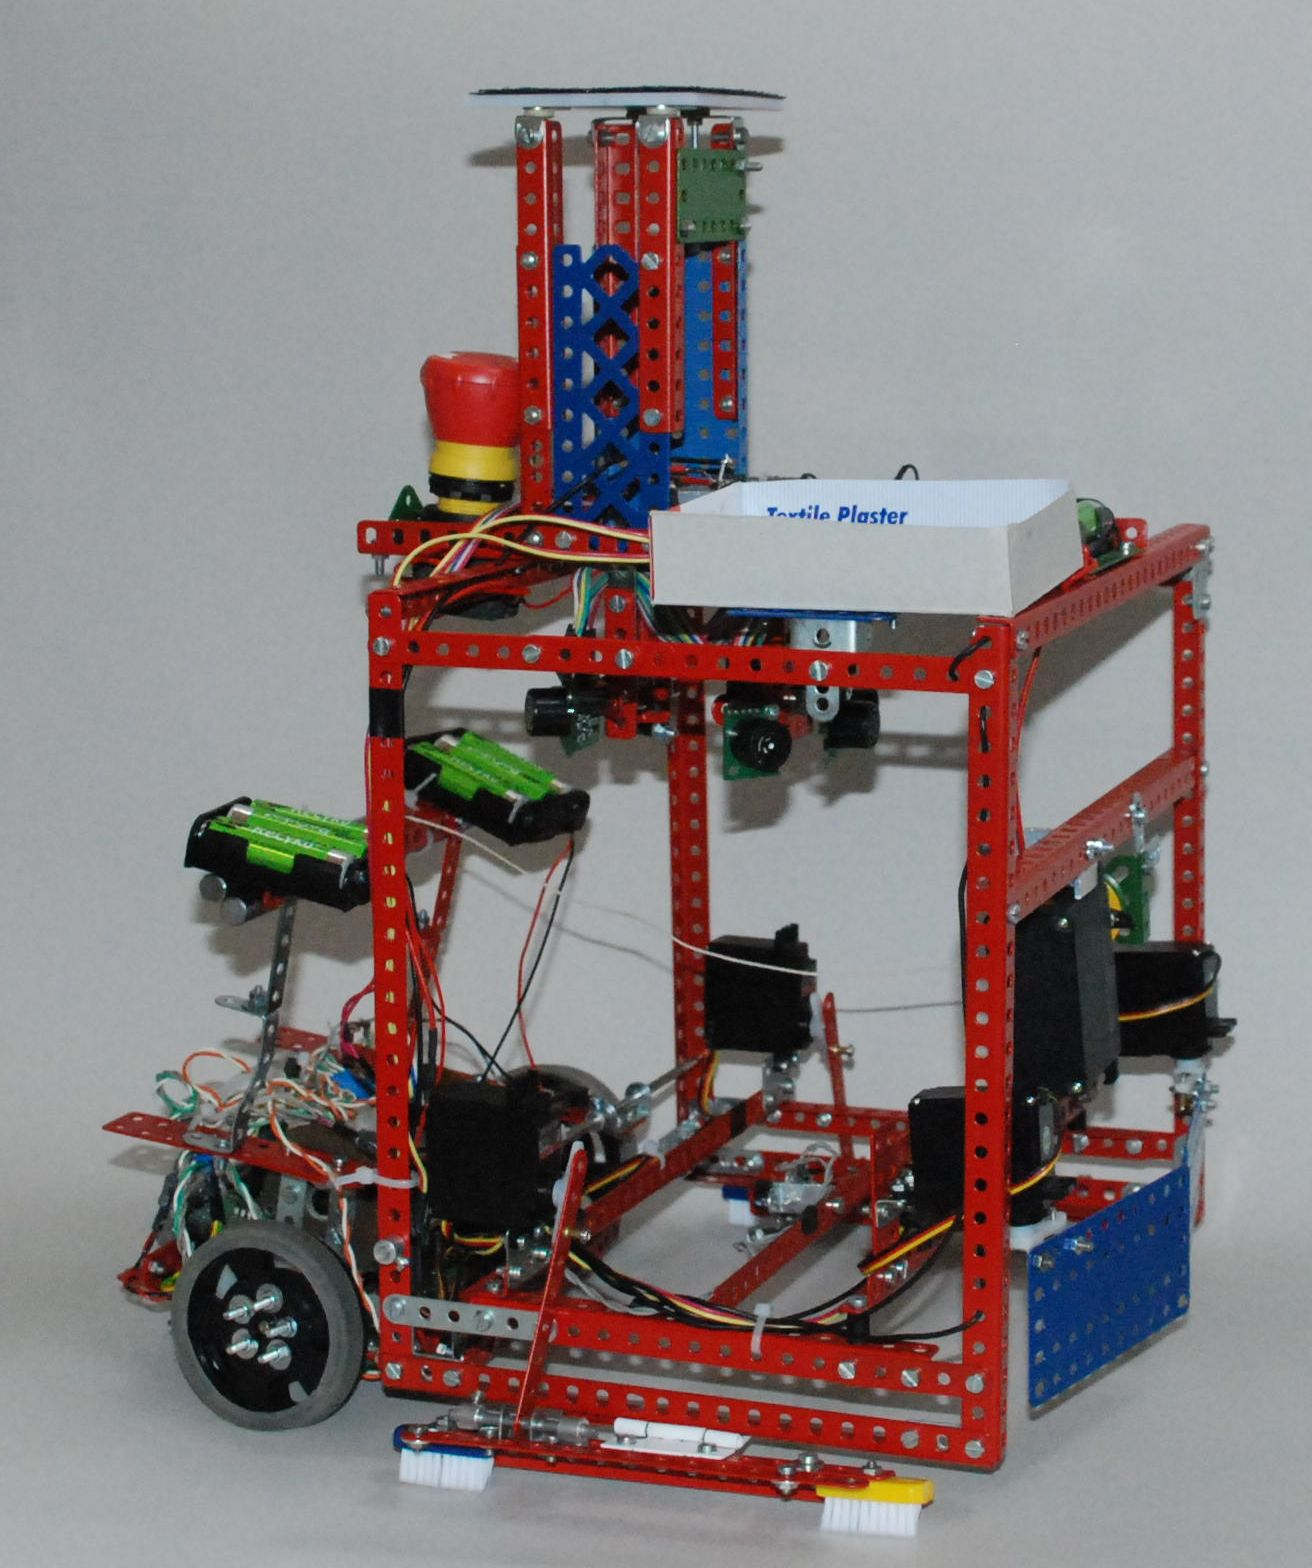
\includegraphics[width=\linewidth]{img/robot.jpg}
    %}
    \end{minipage}
\end{figure}\\
\\{\large \B{Part 1: mechanical frame of the robot}}\\
Body of the robot, along with motors and servomotors, was constructed first. Even in this early phase, my Lorris program was already being used. We needed to test if all the motors and servos work properly and how exactly they behave, so I assembled a small group of widgets in Lorris, which would allows to control the robot via joystick. Several widgets were used, namely \uv{Script}, which was reading data from joystick, calculating the speed values for motors and sending them to the robot. Next, widget \uv{Input}, which contained settings joystick parameters and lastly, 2 widgets \uv{Number} with actual motors̈́' speeds.
\begin{center}
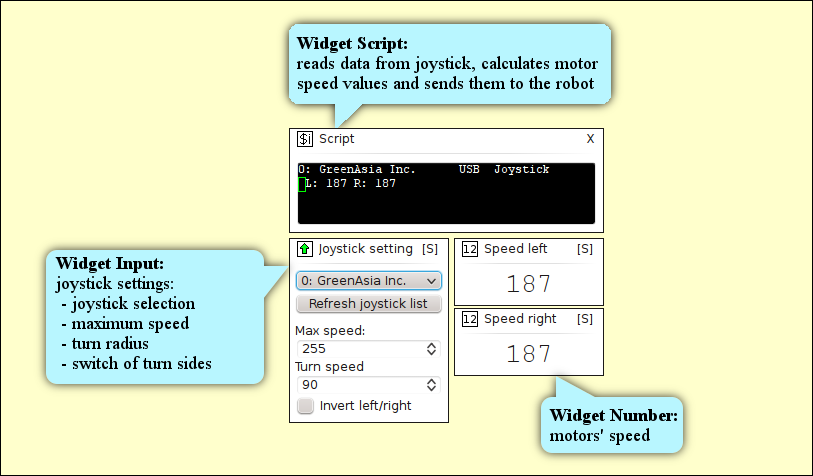
\includegraphics{img/joystick2.png}
\end{center}

\newpage
\enlargethispage{100mm} % zvětší oblast tisku pro tuto stránku   
\voffset = -30mm % posun začátku textu výš
\begin{center}
    \Large \B{APPLICATION EXAMPLE \\Part 2: debugging and ajdusting of sensors}
\end{center}
\vspace{5mm}
When the mechanical frame was complete and tested, all sensors were added to the robot. After that, interface to actually see sensor values was needed, so I created interface for this purpose in Analyzer. It uses mainly \uv{Script}, \uv{Number} \uv{Color} and \uv{Status} widgets. Each and every one of these widgets can be moved around Analyzer's worspace and resized. That makes it possible to place widgets so that their positions coresponds with their real positions on the robot. Top view appears to be ideal for this task.

\vspace{30mm}
\begin{center}
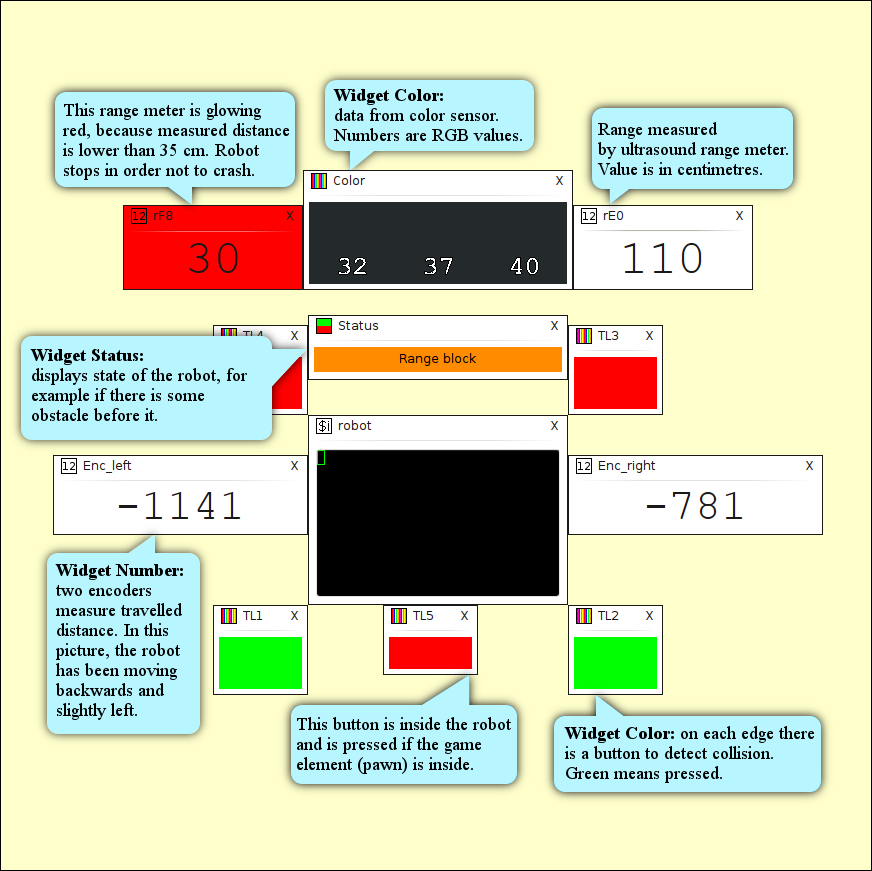
\includegraphics{img/sensors2.png}
\end{center}

\textheight = 380mm
\textwidth = 380mm
\newpage
\enlargethispage{400mm} % zvětší oblast tisku pro tuto stránku   
\begin{landscape}
\voffset = -30mm % posun začátku textu výš
\begin{center}
    \Large \B{APPLICATION EXAMPLE \\Part 3: programování reaktivního chování robota}
\end{center}
\vspace{5mm}
Peak of the developement was programming of it's behavior on the game field. For this occasion, widget \uv{Script} in my Lorris program was used to a large extent. Scripting enviroment which encapsulated robot's basic command sets was created in this widget. These command sets allows us to create more complicated behavioral patterns for the robot. It would be possible to write script for the robot directly, but this enviroment considerably simplified and sped up the developement. Another fact is also worth noticing -- widget \uv{Script} here was used not only to control the robot, but also to improve functionality of the Analyzer tool itself.
 
\begin{center}
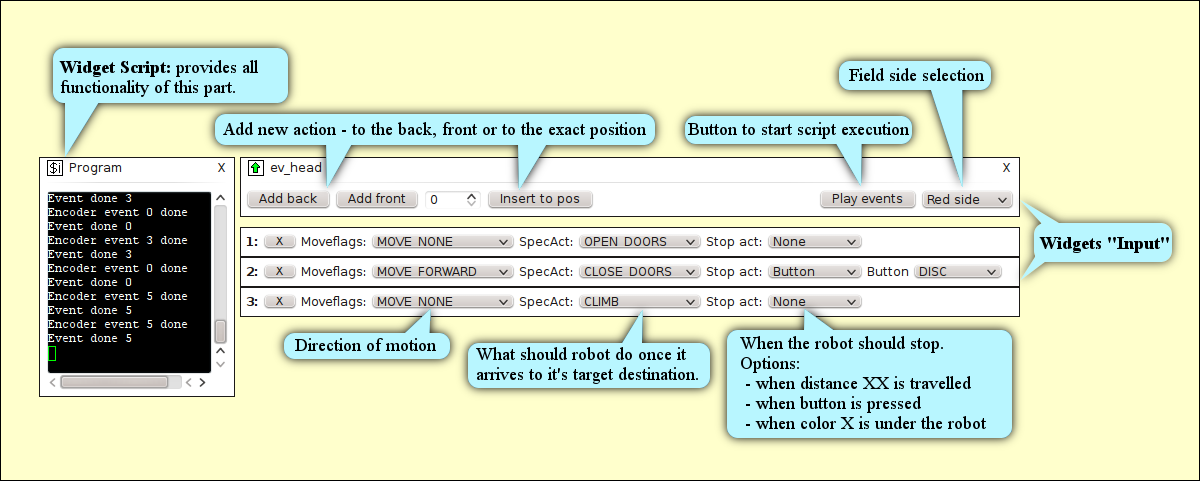
\includegraphics{img/control2.png}
\end{center}

In this example, I use simple \uv{actions}, which are being executed by the robot step by step. Each action has 3 main parameters -- direction of movement, when the robot should stop and what should it do when it arrives at it's target destination. Each action can be changed directly in the scripting enviroment, bypassing the need to re-program robot after every change. All other parts of Lorris are still working, even when the robot is controlled by the script. That makes it possible to keep track of robot's state as well as all his sensors and quickly find source of possible unexpected behavior.
\end{landscape}


\end{document}